\documentclass[twoside]{book}

% Packages required by doxygen
\usepackage{fixltx2e}
\usepackage{calc}
\usepackage{doxygen}
\usepackage[export]{adjustbox} % also loads graphicx
\usepackage{graphicx}
\usepackage[utf8]{inputenc}
\usepackage{makeidx}
\usepackage{multicol}
\usepackage{multirow}
\PassOptionsToPackage{warn}{textcomp}
\usepackage{textcomp}
\usepackage[nointegrals]{wasysym}
\usepackage[table]{xcolor}

% Font selection
\usepackage[T1]{fontenc}
\usepackage[scaled=.90]{helvet}
\usepackage{courier}
\usepackage{amssymb}
\usepackage{sectsty}
\renewcommand{\familydefault}{\sfdefault}
\allsectionsfont{%
  \fontseries{bc}\selectfont%
  \color{darkgray}%
}
\renewcommand{\DoxyLabelFont}{%
  \fontseries{bc}\selectfont%
  \color{darkgray}%
}
\newcommand{\+}{\discretionary{\mbox{\scriptsize$\hookleftarrow$}}{}{}}

% Page & text layout
\usepackage{geometry}
\geometry{%
  a4paper,%
  top=2.5cm,%
  bottom=2.5cm,%
  left=2.5cm,%
  right=2.5cm%
}
\tolerance=750
\hfuzz=15pt
\hbadness=750
\setlength{\emergencystretch}{15pt}
\setlength{\parindent}{0cm}
\setlength{\parskip}{3ex plus 2ex minus 2ex}
\makeatletter
\renewcommand{\paragraph}{%
  \@startsection{paragraph}{4}{0ex}{-1.0ex}{1.0ex}{%
    \normalfont\normalsize\bfseries\SS@parafont%
  }%
}
\renewcommand{\subparagraph}{%
  \@startsection{subparagraph}{5}{0ex}{-1.0ex}{1.0ex}{%
    \normalfont\normalsize\bfseries\SS@subparafont%
  }%
}
\makeatother

% Headers & footers
\usepackage{fancyhdr}
\pagestyle{fancyplain}
\fancyhead[LE]{\fancyplain{}{\bfseries\thepage}}
\fancyhead[CE]{\fancyplain{}{}}
\fancyhead[RE]{\fancyplain{}{\bfseries\leftmark}}
\fancyhead[LO]{\fancyplain{}{\bfseries\rightmark}}
\fancyhead[CO]{\fancyplain{}{}}
\fancyhead[RO]{\fancyplain{}{\bfseries\thepage}}
\fancyfoot[LE]{\fancyplain{}{}}
\fancyfoot[CE]{\fancyplain{}{}}
\fancyfoot[RE]{\fancyplain{}{\bfseries\scriptsize Generated by Doxygen }}
\fancyfoot[LO]{\fancyplain{}{\bfseries\scriptsize Generated by Doxygen }}
\fancyfoot[CO]{\fancyplain{}{}}
\fancyfoot[RO]{\fancyplain{}{}}
\renewcommand{\footrulewidth}{0.4pt}
\renewcommand{\chaptermark}[1]{%
  \markboth{#1}{}%
}
\renewcommand{\sectionmark}[1]{%
  \markright{\thesection\ #1}%
}

% Indices & bibliography
\usepackage{natbib}
\usepackage[titles]{tocloft}
\setcounter{tocdepth}{3}
\setcounter{secnumdepth}{5}
\makeindex

% Hyperlinks (required, but should be loaded last)
\usepackage{ifpdf}
\ifpdf
  \usepackage[pdftex,pagebackref=true]{hyperref}
\else
  \usepackage[ps2pdf,pagebackref=true]{hyperref}
\fi
\hypersetup{%
  colorlinks=true,%
  linkcolor=blue,%
  citecolor=blue,%
  unicode%
}

% Custom commands
\newcommand{\clearemptydoublepage}{%
  \newpage{\pagestyle{empty}\cleardoublepage}%
}

\usepackage{caption}
\captionsetup{labelsep=space,justification=centering,font={bf},singlelinecheck=off,skip=4pt,position=top}

%===== C O N T E N T S =====

\begin{document}

% Titlepage & ToC
\hypersetup{pageanchor=false,
             bookmarksnumbered=true,
             pdfencoding=unicode
            }
\pagenumbering{roman}
\begin{titlepage}
\vspace*{7cm}
\begin{center}%
{\Large My Project }\\
\vspace*{1cm}
{\large Generated by Doxygen 1.8.11}\\
\end{center}
\end{titlepage}
\clearemptydoublepage
\tableofcontents
\clearemptydoublepage
\pagenumbering{arabic}
\hypersetup{pageanchor=true}

%--- Begin generated contents ---
\chapter{Namespace Index}
\section{Namespace List}
Here is a list of all documented namespaces with brief descriptions\+:\begin{DoxyCompactList}
\item\contentsline{section}{\hyperlink{namespacemain__savitch__14}{main\+\_\+savitch\+\_\+14} }{\pageref{namespacemain__savitch__14}}{}
\end{DoxyCompactList}

\chapter{Hierarchical Index}
\section{Class Hierarchy}
This inheritance list is sorted roughly, but not completely, alphabetically\+:\begin{DoxyCompactList}
\item \contentsline{section}{main\+\_\+savitch\+\_\+14\+:\+:game}{\pageref{classmain__savitch__14_1_1game}}{}
\begin{DoxyCompactList}
<<<<<<< HEAD
\item \contentsline{section}{main\+\_\+savitch\+\_\+14\+:\+:Othello}{\pageref{classmain__savitch__14_1_1Othello}}{}
=======
\item \contentsline{section}{main\+\_\+savitch\+\_\+14\+:\+:Othello}{\pageref{classmain__savitch__14_1_1_othello}}{}
>>>>>>> 731e3373baaf3f8b497d3ebf8294d88f708cd837
\end{DoxyCompactList}
\item \contentsline{section}{piece}{\pageref{classpiece}}{}
\end{DoxyCompactList}

\chapter{Class Index}
\section{Class List}
Here are the classes, structs, unions and interfaces with brief descriptions\+:\begin{DoxyCompactList}
\item\contentsline{section}{\hyperlink{classCollege}{College} }{\pageref{classCollege}}{}
\item\contentsline{section}{\hyperlink{classcourse}{course} }{\pageref{classcourse}}{}
\item\contentsline{section}{\hyperlink{classnode}{node} }{\pageref{classnode}}{}
\item\contentsline{section}{\hyperlink{classTarray}{Tarray$<$ T $>$} }{\pageref{classTarray}}{}
\end{DoxyCompactList}

\chapter{File Index}
\section{File List}
Here is a list of all documented files with brief descriptions\+:\begin{DoxyCompactList}
\item\contentsline{section}{\hyperlink{college_8cc}{college.\+cc} \\*Implementation file for college class }{\pageref{college_8cc}}{}
\item\contentsline{section}{\hyperlink{college_8h}{college.\+h} \\*Header file for college class }{\pageref{college_8h}}{}
\item\contentsline{section}{\hyperlink{collegemain_8cc}{collegemain.\+cc} \\*Main for college container }{\pageref{collegemain_8cc}}{}
\item\contentsline{section}{\hyperlink{course_8cc}{course.\+cc} \\*Implementation for course class }{\pageref{course_8cc}}{}
\item\contentsline{section}{\hyperlink{course_8h}{course.\+h} \\*Header file for course class }{\pageref{course_8h}}{}
\item\contentsline{section}{\hyperlink{node_8h}{node.\+h} \\*Implementation for node class }{\pageref{node_8h}}{}
\item\contentsline{section}{\hyperlink{tarray_8h}{tarray.\+h} \\*Implementation for \hyperlink{classTarray}{Tarray} class }{\pageref{tarray_8h}}{}
\end{DoxyCompactList}

\chapter{Namespace Documentation}
\hypertarget{namespacemain__savitch__14}{}\section{main\+\_\+savitch\+\_\+14 Namespace Reference}
\label{namespacemain__savitch__14}\index{main\+\_\+savitch\+\_\+14@{main\+\_\+savitch\+\_\+14}}
\subsection*{Classes}
\begin{DoxyCompactItemize}
\item 
class \hyperlink{classmain__savitch__14_1_1game}{game}
\item 
class \hyperlink{classmain__savitch__14_1_1Othello}{Othello}
\end{DoxyCompactItemize}


\subsection{Detailed Description}
File name\+: \hyperlink{game_8h_source}{game.\+h} Names\+: Marcus Mc\+Kinley, Lydia Shiffler, Josh Wright, Eric Hahn Date\+: 2/25/2018 Description\+: This is the game class. It can be used to make many games.

File Name\+: othello.\+cc Names\+: Lydia Shiffler, Marcus Mc\+Kinley, Josh Wright, Eric Hahn Date\+: 2/25/18 Description\+: the othello.\+cc gives the functions to play the game othello and gives the different moves possible 
\chapter{Class Documentation}
\hypertarget{classmain__savitch__14_1_1game}{}\section{main\+\_\+savitch\+\_\+14\+:\+:game Class Reference}
\label{classmain__savitch__14_1_1game}\index{main\+\_\+savitch\+\_\+14\+::game@{main\+\_\+savitch\+\_\+14\+::game}}


Inheritance diagram for main\+\_\+savitch\+\_\+14\+:\+:game\+:
% FIG 0
\subsection*{Public Types}
\begin{DoxyCompactItemize}
\item 
enum {\bfseries who} \{ {\bfseries H\+U\+M\+AN}, 
{\bfseries N\+E\+U\+T\+R\+AL}, 
{\bfseries C\+O\+M\+P\+U\+T\+ER}
 \}\hypertarget{classmain__savitch__14_1_1game_a4fe20fb287f809ae2b68e28e4ccba634}{}\label{classmain__savitch__14_1_1game_a4fe20fb287f809ae2b68e28e4ccba634}

\end{DoxyCompactItemize}
\subsection*{Public Member Functions}
\begin{DoxyCompactItemize}
\item 
who \hyperlink{classmain__savitch__14_1_1game_a4dbeaddb78059f7c5dcbf5cc4e026317}{play} ()
\end{DoxyCompactItemize}
\subsection*{Protected Member Functions}
\begin{DoxyCompactItemize}
\item 
virtual void \hyperlink{classmain__savitch__14_1_1game_ab8b87c3a1b68634861a8c0ed2b9f1992}{display\+\_\+message} (const std\+::string \&message) const 
\begin{DoxyCompactList}\small\item\em display\+\_\+message displays the message from the game \end{DoxyCompactList}\item 
virtual std\+::string \hyperlink{classmain__savitch__14_1_1game_a1265f262f5a15bca5b532e6e97d13089}{get\+\_\+user\+\_\+move} () const 
\item 
virtual who {\bfseries last\+\_\+mover} () const \hypertarget{classmain__savitch__14_1_1game_a38d435da6aadc192ac10160b26ea0cc1}{}\label{classmain__savitch__14_1_1game_a38d435da6aadc192ac10160b26ea0cc1}

\item 
virtual int {\bfseries moves\+\_\+completed} () const \hypertarget{classmain__savitch__14_1_1game_aee677d1ef52c35474cb7c6071bb71749}{}\label{classmain__savitch__14_1_1game_aee677d1ef52c35474cb7c6071bb71749}

\item 
virtual who {\bfseries next\+\_\+mover} () const \hypertarget{classmain__savitch__14_1_1game_a0d445fdec3201c91c145ee2763e08922}{}\label{classmain__savitch__14_1_1game_a0d445fdec3201c91c145ee2763e08922}

\item 
virtual who {\bfseries opposite} (who player) const \hypertarget{classmain__savitch__14_1_1game_ae38d001e92ebe46e1a1433e41446c7ab}{}\label{classmain__savitch__14_1_1game_ae38d001e92ebe46e1a1433e41446c7ab}

\item 
virtual void {\bfseries counting\+Pieces} ()=0\hypertarget{classmain__savitch__14_1_1game_a5954eccb6abf1ae900ad853ad2af99fa}{}\label{classmain__savitch__14_1_1game_a5954eccb6abf1ae900ad853ad2af99fa}

\item 
virtual void {\bfseries whos\+Turn} ()=0\hypertarget{classmain__savitch__14_1_1game_a98190a2bf784ce0f20533475754d136d}{}\label{classmain__savitch__14_1_1game_a98190a2bf784ce0f20533475754d136d}

\item 
virtual who \hyperlink{classmain__savitch__14_1_1game_a081611c42aa66b4d91bbefeec47c7c4e}{winning} () const 
\begin{DoxyCompactList}\small\item\em Winning returns the user that is winning. \end{DoxyCompactList}\item 
virtual void \hyperlink{classmain__savitch__14_1_1game_a20597d0caa907aea47b27fed8be3759b}{make\+\_\+move} (const std\+::string \&move)\hypertarget{classmain__savitch__14_1_1game_a20597d0caa907aea47b27fed8be3759b}{}\label{classmain__savitch__14_1_1game_a20597d0caa907aea47b27fed8be3759b}

\begin{DoxyCompactList}\small\item\em Have the next player make a specified move\+: \end{DoxyCompactList}\item 
virtual void {\bfseries restart} ()\hypertarget{classmain__savitch__14_1_1game_ad521a7d78e7c163a0bc28b709f0d45fd}{}\label{classmain__savitch__14_1_1game_ad521a7d78e7c163a0bc28b709f0d45fd}

\item 
virtual \hyperlink{classmain__savitch__14_1_1game}{game} $\ast$ {\bfseries clone} () const =0\hypertarget{classmain__savitch__14_1_1game_a7b663057f59210dd52738facfc40d959}{}\label{classmain__savitch__14_1_1game_a7b663057f59210dd52738facfc40d959}

\item 
virtual void {\bfseries compute\+\_\+moves} (std\+::queue$<$ std\+::string $>$ \&moves) const =0\hypertarget{classmain__savitch__14_1_1game_a2c0c049f5861026d0f639b5837889b7a}{}\label{classmain__savitch__14_1_1game_a2c0c049f5861026d0f639b5837889b7a}

\item 
virtual void {\bfseries display\+\_\+status} () const =0\hypertarget{classmain__savitch__14_1_1game_ac8205178922c49bab2865187e834b726}{}\label{classmain__savitch__14_1_1game_ac8205178922c49bab2865187e834b726}

\item 
virtual int {\bfseries evaluate} () const =0\hypertarget{classmain__savitch__14_1_1game_a9b9c8c5e9aa57c9a430f20b87cb047aa}{}\label{classmain__savitch__14_1_1game_a9b9c8c5e9aa57c9a430f20b87cb047aa}

\item 
virtual bool {\bfseries is\+\_\+game\+\_\+over} () const =0\hypertarget{classmain__savitch__14_1_1game_a49eed20648918b03fd3e2cf78987b3d1}{}\label{classmain__savitch__14_1_1game_a49eed20648918b03fd3e2cf78987b3d1}

\item 
virtual bool {\bfseries is\+\_\+legal} (const std\+::string \&move) const =0\hypertarget{classmain__savitch__14_1_1game_ad38351422ca1ee3ae58440c1c6b36b30}{}\label{classmain__savitch__14_1_1game_ad38351422ca1ee3ae58440c1c6b36b30}

\end{DoxyCompactItemize}
\subsection*{Protected Attributes}
\begin{DoxyCompactItemize}
\item 
int {\bfseries move\+\_\+number}\hypertarget{classmain__savitch__14_1_1game_ac4c296f4370d8e5bb5ea74b638fb827d}{}\label{classmain__savitch__14_1_1game_ac4c296f4370d8e5bb5ea74b638fb827d}

\end{DoxyCompactItemize}


\subsection{Member Function Documentation}
\index{main\+\_\+savitch\+\_\+14\+::game@{main\+\_\+savitch\+\_\+14\+::game}!display\+\_\+message@{display\+\_\+message}}
\index{display\+\_\+message@{display\+\_\+message}!main\+\_\+savitch\+\_\+14\+::game@{main\+\_\+savitch\+\_\+14\+::game}}
\subsubsection[{\texorpdfstring{display\+\_\+message(const std\+::string \&message) const }{display_message(const std::string &message) const }}]{\setlength{\rightskip}{0pt plus 5cm}void main\+\_\+savitch\+\_\+14\+::game\+::display\+\_\+message (
\begin{DoxyParamCaption}
\item[{const std\+::string \&}]{message}
\end{DoxyParamCaption}
) const\hspace{0.3cm}{\ttfamily [protected]}, {\ttfamily [virtual]}}\hypertarget{classmain__savitch__14_1_1game_ab8b87c3a1b68634861a8c0ed2b9f1992}{}\label{classmain__savitch__14_1_1game_ab8b87c3a1b68634861a8c0ed2b9f1992}


display\+\_\+message displays the message from the game 


\begin{DoxyParams}{Parameters}
{\em const} & string\& message \\
\hline
\end{DoxyParams}
\begin{DoxyReturn}{Returns}
n/a 
\end{DoxyReturn}
\index{main\+\_\+savitch\+\_\+14\+::game@{main\+\_\+savitch\+\_\+14\+::game}!get\+\_\+user\+\_\+move@{get\+\_\+user\+\_\+move}}
\index{get\+\_\+user\+\_\+move@{get\+\_\+user\+\_\+move}!main\+\_\+savitch\+\_\+14\+::game@{main\+\_\+savitch\+\_\+14\+::game}}
\subsubsection[{\texorpdfstring{get\+\_\+user\+\_\+move() const }{get_user_move() const }}]{\setlength{\rightskip}{0pt plus 5cm}string main\+\_\+savitch\+\_\+14\+::game\+::get\+\_\+user\+\_\+move (
\begin{DoxyParamCaption}
{}
\end{DoxyParamCaption}
) const\hspace{0.3cm}{\ttfamily [protected]}, {\ttfamily [virtual]}}\hypertarget{classmain__savitch__14_1_1game_a1265f262f5a15bca5b532e6e97d13089}{}\label{classmain__savitch__14_1_1game_a1265f262f5a15bca5b532e6e97d13089}

\begin{DoxyParams}{Parameters}
{\em n/a} & \\
\hline
\end{DoxyParams}
\begin{DoxyReturn}{Returns}
string get\+\_\+user\+\_\+move displays a message to either tell the user to press S if $\ast$he/she cannot move, or tells them that it is their move 
\end{DoxyReturn}
\index{main\+\_\+savitch\+\_\+14\+::game@{main\+\_\+savitch\+\_\+14\+::game}!play@{play}}
\index{play@{play}!main\+\_\+savitch\+\_\+14\+::game@{main\+\_\+savitch\+\_\+14\+::game}}
\subsubsection[{\texorpdfstring{play()}{play()}}]{\setlength{\rightskip}{0pt plus 5cm}game\+::who main\+\_\+savitch\+\_\+14\+::game\+::play (
\begin{DoxyParamCaption}
{}
\end{DoxyParamCaption}
)}\hypertarget{classmain__savitch__14_1_1game_a4dbeaddb78059f7c5dcbf5cc4e026317}{}\label{classmain__savitch__14_1_1game_a4dbeaddb78059f7c5dcbf5cc4e026317}

\begin{DoxyParams}{Parameters}
{\em n/a} & \\
\hline
\end{DoxyParams}
\begin{DoxyReturn}{Returns}
game\+::who The play function should not be overridden. It plays one round of the game, with the human player moving first and the computer second. The return value is the winner of the game (or N\+E\+U\+T\+R\+AL for a tie). 
\end{DoxyReturn}
\index{main\+\_\+savitch\+\_\+14\+::game@{main\+\_\+savitch\+\_\+14\+::game}!winning@{winning}}
\index{winning@{winning}!main\+\_\+savitch\+\_\+14\+::game@{main\+\_\+savitch\+\_\+14\+::game}}
\subsubsection[{\texorpdfstring{winning() const }{winning() const }}]{\setlength{\rightskip}{0pt plus 5cm}game\+::who main\+\_\+savitch\+\_\+14\+::game\+::winning (
\begin{DoxyParamCaption}
{}
\end{DoxyParamCaption}
) const\hspace{0.3cm}{\ttfamily [protected]}, {\ttfamily [virtual]}}\hypertarget{classmain__savitch__14_1_1game_a081611c42aa66b4d91bbefeec47c7c4e}{}\label{classmain__savitch__14_1_1game_a081611c42aa66b4d91bbefeec47c7c4e}


Winning returns the user that is winning. 


\begin{DoxyParams}{Parameters}
{\em n/a} & \\
\hline
\end{DoxyParams}
\begin{DoxyReturn}{Returns}
game\+::who 
\end{DoxyReturn}


Reimplemented in \hyperlink{classmain__savitch__14_1_1Othello_a8934d1b63f73c03dae9629dbe03955d7}{main\+\_\+savitch\+\_\+14\+::\+Othello}.



The documentation for this class was generated from the following files\+:\begin{DoxyCompactItemize}
\item 
game.\+h\item 
game.\+cc\end{DoxyCompactItemize}

\hypertarget{classmain__savitch__14_1_1_othello}{}\section{main\+\_\+savitch\+\_\+14\+:\+:Othello Class Reference}
\label{classmain__savitch__14_1_1_othello}\index{main\+\_\+savitch\+\_\+14\+::\+Othello@{main\+\_\+savitch\+\_\+14\+::\+Othello}}
Inheritance diagram for main\+\_\+savitch\+\_\+14\+:\+:Othello\+:\begin{figure}[H]
\begin{center}
\leavevmode
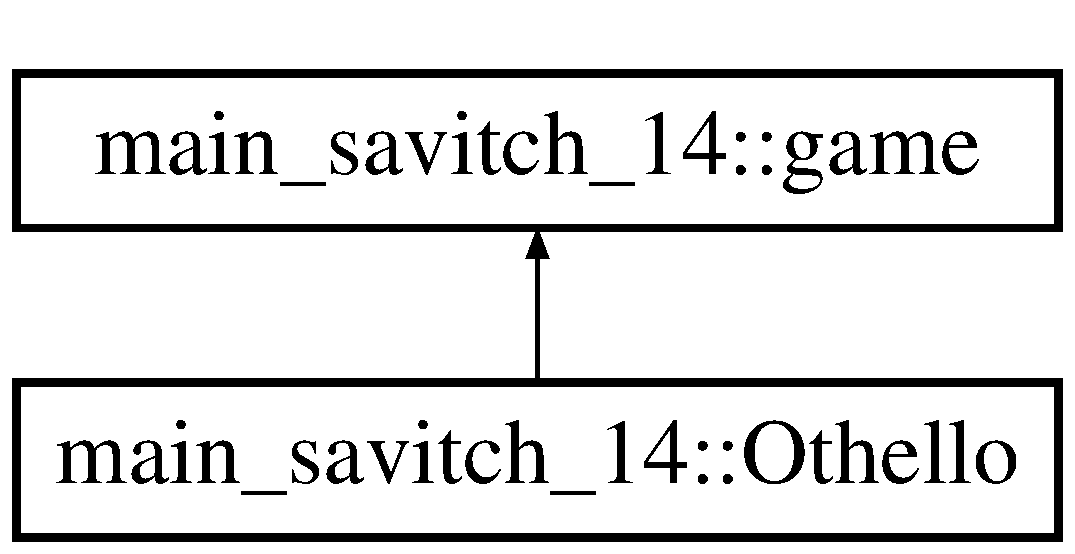
\includegraphics[height=2.000000cm]{classmain__savitch__14_1_1_othello}
\end{center}
\end{figure}
\subsection*{Public Member Functions}
\begin{DoxyCompactItemize}
\item 
\mbox{\Hypertarget{classmain__savitch__14_1_1_othello_ab01a4f7aba130133221a11224905e8ce}\label{classmain__savitch__14_1_1_othello_ab01a4f7aba130133221a11224905e8ce}} 
void {\bfseries display\+\_\+status} () const
\item 
\mbox{\Hypertarget{classmain__savitch__14_1_1_othello_a57ae44590de8d683592f186ed6bd25b0}\label{classmain__savitch__14_1_1_othello_a57ae44590de8d683592f186ed6bd25b0}} 
int {\bfseries evaluate} () const
\item 
\mbox{\Hypertarget{classmain__savitch__14_1_1_othello_a540c8b0030e429e0ac30f07e9e8868ec}\label{classmain__savitch__14_1_1_othello_a540c8b0030e429e0ac30f07e9e8868ec}} 
bool {\bfseries is\+\_\+game\+\_\+over} () const
\item 
\mbox{\Hypertarget{classmain__savitch__14_1_1_othello_a74ac0d4e6399167037dfc708efdb9033}\label{classmain__savitch__14_1_1_othello_a74ac0d4e6399167037dfc708efdb9033}} 
bool {\bfseries is\+\_\+legal} (const string \&move) const
\item 
\mbox{\Hypertarget{classmain__savitch__14_1_1_othello_a1066b280efa5cb41039585669282fe06}\label{classmain__savitch__14_1_1_othello_a1066b280efa5cb41039585669282fe06}} 
void {\bfseries make\+\_\+move} (const string \&move)
\item 
\mbox{\Hypertarget{classmain__savitch__14_1_1_othello_abf872b8074bfa4c04119317dc3b39af2}\label{classmain__savitch__14_1_1_othello_abf872b8074bfa4c04119317dc3b39af2}} 
void {\bfseries restart} ()
\item 
\mbox{\Hypertarget{classmain__savitch__14_1_1_othello_a3177234195a490eef52343d957e64b5d}\label{classmain__savitch__14_1_1_othello_a3177234195a490eef52343d957e64b5d}} 
void {\bfseries make\+\_\+skips} ()
\item 
\mbox{\Hypertarget{classmain__savitch__14_1_1_othello_a19f49edfbe82b84922877e00bc854ed8}\label{classmain__savitch__14_1_1_othello_a19f49edfbe82b84922877e00bc854ed8}} 
void {\bfseries counting\+Pieces} ()
\item 
\mbox{\Hypertarget{classmain__savitch__14_1_1_othello_a21440dbb4511812a76c578a5f546710b}\label{classmain__savitch__14_1_1_othello_a21440dbb4511812a76c578a5f546710b}} 
void {\bfseries whos\+Turn} ()
\item 
\mbox{\Hypertarget{classmain__savitch__14_1_1_othello_a7a5f8495f1a61f6e7b3968e919013c18}\label{classmain__savitch__14_1_1_othello_a7a5f8495f1a61f6e7b3968e919013c18}} 
\mbox{\hyperlink{classmain__savitch__14_1_1game}{game}} $\ast$ {\bfseries clone} () const
\item 
\mbox{\Hypertarget{classmain__savitch__14_1_1_othello_a921d4ffa277b0250f187f20b9598ebb1}\label{classmain__savitch__14_1_1_othello_a921d4ffa277b0250f187f20b9598ebb1}} 
void {\bfseries compute\+\_\+moves} (std\+::queue$<$ std\+::string $>$ \&moves) const
\item 
\mbox{\Hypertarget{classmain__savitch__14_1_1_othello_a4ea78b18eea66c944c0a9356349e0fd4}\label{classmain__savitch__14_1_1_othello_a4ea78b18eea66c944c0a9356349e0fd4}} 
who {\bfseries winning} () const
\end{DoxyCompactItemize}
\subsection*{Protected Attributes}
\begin{DoxyCompactItemize}
\item 
\mbox{\Hypertarget{classmain__savitch__14_1_1_othello_a2eed818925f68d5678b78107a3298138}\label{classmain__savitch__14_1_1_othello_a2eed818925f68d5678b78107a3298138}} 
int {\bfseries black}
\item 
\mbox{\Hypertarget{classmain__savitch__14_1_1_othello_a7d5f59b1e581ed7a8145debeecf4f310}\label{classmain__savitch__14_1_1_othello_a7d5f59b1e581ed7a8145debeecf4f310}} 
int {\bfseries white}
\item 
\mbox{\Hypertarget{classmain__savitch__14_1_1_othello_a85d4ce17512d8dbf85a313a27eea0644}\label{classmain__savitch__14_1_1_othello_a85d4ce17512d8dbf85a313a27eea0644}} 
int {\bfseries skips}
\item 
\mbox{\Hypertarget{classmain__savitch__14_1_1_othello_a15045e3e94c34afe08240885e230d502}\label{classmain__savitch__14_1_1_othello_a15045e3e94c34afe08240885e230d502}} 
int {\bfseries open\+Spots}
\item 
\mbox{\Hypertarget{classmain__savitch__14_1_1_othello_a98fbc46241d2f5e05ccb4b66f11535bf}\label{classmain__savitch__14_1_1_othello_a98fbc46241d2f5e05ccb4b66f11535bf}} 
int {\bfseries b}
\item 
\mbox{\Hypertarget{classmain__savitch__14_1_1_othello_a1b11c5fe33e30a94ed39e8cb55caf37e}\label{classmain__savitch__14_1_1_othello_a1b11c5fe33e30a94ed39e8cb55caf37e}} 
int {\bfseries w}
\end{DoxyCompactItemize}
\subsection*{Additional Inherited Members}


The documentation for this class was generated from the following files\+:\begin{DoxyCompactItemize}
\item 
othello.\+h\item 
othello.\+cc\end{DoxyCompactItemize}

\hypertarget{classpiece}{}\section{piece Class Reference}
\label{classpiece}\index{piece@{piece}}
\subsection*{Public Member Functions}
\begin{DoxyCompactItemize}
\item 
void {\bfseries flip} ()\hypertarget{classpiece_ab898c5827a5859e4cddc9d61a814a873}{}\label{classpiece_ab898c5827a5859e4cddc9d61a814a873}

\item 
bool {\bfseries is\+\_\+blank} () const \hypertarget{classpiece_af8e5afd9e1eb6b367c7da643c94c7113}{}\label{classpiece_af8e5afd9e1eb6b367c7da643c94c7113}

\item 
bool {\bfseries is\+\_\+black} () const \hypertarget{classpiece_abb229bd7452561f1f3aa794e5561aa60}{}\label{classpiece_abb229bd7452561f1f3aa794e5561aa60}

\item 
bool {\bfseries is\+\_\+white} () const \hypertarget{classpiece_a229a0c4b29e449350b2c3ba019e6c9a9}{}\label{classpiece_a229a0c4b29e449350b2c3ba019e6c9a9}

\item 
void {\bfseries set\+\_\+white} ()\hypertarget{classpiece_a31480899f2a591fdb22d97933303e19d}{}\label{classpiece_a31480899f2a591fdb22d97933303e19d}

\item 
void {\bfseries set\+\_\+black} ()\hypertarget{classpiece_a273d63d07b6ea973b2fc4f7e1b56ea10}{}\label{classpiece_a273d63d07b6ea973b2fc4f7e1b56ea10}

\end{DoxyCompactItemize}
\subsection*{Private Attributes}
\begin{DoxyCompactItemize}
\item 
color {\bfseries the\+Color}\hypertarget{classpiece_a708f7114877b8c4864e2b8e605794f4f}{}\label{classpiece_a708f7114877b8c4864e2b8e605794f4f}

\end{DoxyCompactItemize}


The documentation for this class was generated from the following file\+:\begin{DoxyCompactItemize}
\item 
/home/marcus/cs3560/\+Assignment-\/6/\+Sample\+\_\+student\+\_\+project/piece.\+h\end{DoxyCompactItemize}

\chapter{File Documentation}
\hypertarget{colors_8h}{}\section{colors.\+h File Reference}
\label{colors_8h}\index{colors.\+h@{colors.\+h}}
{\ttfamily \#include $<$string$>$}\\*
Include dependency graph for colors.\+h\+:

\hypertarget{game_8cc}{}\section{game.\+cc File Reference}
\label{game_8cc}\index{game.\+cc@{game.\+cc}}
{\ttfamily \#include $<$cassert$>$}\\*
{\ttfamily \#include $<$climits$>$}\\*
{\ttfamily \#include $<$iostream$>$}\\*
{\ttfamily \#include $<$queue$>$}\\*
{\ttfamily \#include $<$string$>$}\\*
{\ttfamily \#include \char`\"{}game.\+h\char`\"{}}\\*
Include dependency graph for game.\+cc\+:
% FIG 0
\subsection*{Namespaces}
\begin{DoxyCompactItemize}
\item 
 \hyperlink{namespacemain__savitch__14}{main\+\_\+savitch\+\_\+14}
\end{DoxyCompactItemize}

\hypertarget{game_8h}{}\section{game.\+h File Reference}
\label{game_8h}\index{game.\+h@{game.\+h}}
{\ttfamily \#include $<$queue$>$}\\*
{\ttfamily \#include $<$string$>$}\\*
Include dependency graph for game.\+h\+:
% FIG 0
This graph shows which files directly or indirectly include this file\+:
% FIG 1
\subsection*{Classes}
\begin{DoxyCompactItemize}
\item 
class \hyperlink{classmain__savitch__14_1_1game}{main\+\_\+savitch\+\_\+14\+::game}
\end{DoxyCompactItemize}
\subsection*{Namespaces}
\begin{DoxyCompactItemize}
\item 
 \hyperlink{namespacemain__savitch__14}{main\+\_\+savitch\+\_\+14}
\end{DoxyCompactItemize}

\hypertarget{main_8cc}{}\section{main.\+cc File Reference}
\label{main_8cc}\index{main.\+cc@{main.\+cc}}
{\ttfamily \#include \char`\"{}game.\+h\char`\"{}}\\*
{\ttfamily \#include \char`\"{}othello.\+h\char`\"{}}\\*
Include dependency graph for main.\+cc\+:
% FIG 0
\subsection*{Functions}
\begin{DoxyCompactItemize}
\item 
int \hyperlink{main_8cc_ae66f6b31b5ad750f1fe042a706a4e3d4}{main} ()
\end{DoxyCompactItemize}


\subsection{Detailed Description}
\begin{DoxyAuthor}{Author}
Eric Hahn, Marcus Mc\+Kinley, Lydia Shiffler, Josh Wright
\end{DoxyAuthor}
Description\+: Driver program using \char`\"{}othello.\+h\char`\"{} and \char`\"{}game.\+h\char`\"{} to play a game of Othello with the user. Date\+: 2/25/2018 

\subsection{Function Documentation}
\index{main.\+cc@{main.\+cc}!main@{main}}
\index{main@{main}!main.\+cc@{main.\+cc}}
\subsubsection[{\texorpdfstring{main()}{main()}}]{\setlength{\rightskip}{0pt plus 5cm}int main (
\begin{DoxyParamCaption}
{}
\end{DoxyParamCaption}
)}\hypertarget{main_8cc_ae66f6b31b5ad750f1fe042a706a4e3d4}{}\label{main_8cc_ae66f6b31b5ad750f1fe042a706a4e3d4}
Create an Othello game from \char`\"{}othello.\+h\char`\"{} and continue to run it until the user specifies otherwise. The othello class uses the \char`\"{}game.\+h\char`\"{} class to create the board and control the game.


\begin{DoxyParams}{Parameters}
{\em n/a} & \\
\hline
\end{DoxyParams}
\begin{DoxyReturn}{Returns}
int 
\end{DoxyReturn}

\hypertarget{othello_8cc}{}\section{othello.\+cc File Reference}
\label{othello_8cc}\index{othello.\+cc@{othello.\+cc}}
{\ttfamily \#include \char`\"{}othello.\+h\char`\"{}}\\*
Include dependency graph for othello.\+cc\+:
% FIG 0
\subsection*{Namespaces}
\begin{DoxyCompactItemize}
\item 
 \hyperlink{namespacemain__savitch__14}{main\+\_\+savitch\+\_\+14}
\end{DoxyCompactItemize}

\hypertarget{othello_8h}{}\section{othello.\+h File Reference}
\label{othello_8h}\index{othello.\+h@{othello.\+h}}
{\ttfamily \#include \char`\"{}game.\+h\char`\"{}}\\*
{\ttfamily \#include \char`\"{}piece.\+h\char`\"{}}\\*
{\ttfamily \#include \char`\"{}colors.\+h\char`\"{}}\\*
{\ttfamily \#include $<$iostream$>$}\\*
Include dependency graph for othello.\+h\+:
% FIG 0
This graph shows which files directly or indirectly include this file\+:
% FIG 1
\subsection*{Classes}
\begin{DoxyCompactItemize}
\item 
class \hyperlink{classmain__savitch__14_1_1_othello}{main\+\_\+savitch\+\_\+14\+::\+Othello}
\end{DoxyCompactItemize}
\subsection*{Namespaces}
\begin{DoxyCompactItemize}
\item 
 \hyperlink{namespacemain__savitch__14}{main\+\_\+savitch\+\_\+14}
\end{DoxyCompactItemize}

\hypertarget{piece_8h}{}\section{piece.\+h File Reference}
\label{piece_8h}\index{piece.\+h@{piece.\+h}}
This graph shows which files directly or indirectly include this file\+:
% FIG 0
\subsection*{Classes}
\begin{DoxyCompactItemize}
\item 
class \hyperlink{classpiece}{piece}
\end{DoxyCompactItemize}
\subsection*{Enumerations}
\begin{DoxyCompactItemize}
\item 
enum \hyperlink{piece_8h_a37dbdc30935031c05304482e1be89d8f}{color} \{ \hyperlink{piece_8h_a37dbdc30935031c05304482e1be89d8fa775364fe1f3fffe99686bf6d572a7370}{black}, 
\hyperlink{piece_8h_a37dbdc30935031c05304482e1be89d8fade7bfe6c82a2aaaee276f752cdadf3a9}{white}, 
\hyperlink{piece_8h_a37dbdc30935031c05304482e1be89d8fa77d6578fc94ca0d1dda80da62f41af0e}{blank}
 \}
\end{DoxyCompactItemize}


\subsection{Enumeration Type Documentation}
\index{piece.\+h@{piece.\+h}!color@{color}}
\index{color@{color}!piece.\+h@{piece.\+h}}
\subsubsection[{\texorpdfstring{color}{color}}]{\setlength{\rightskip}{0pt plus 5cm}enum {\bf color}}\hypertarget{piece_8h_a37dbdc30935031c05304482e1be89d8f}{}\label{piece_8h_a37dbdc30935031c05304482e1be89d8f}
\begin{Desc}
\item[Enumerator]\par
\begin{description}
\index{black@{black}!piece.\+h@{piece.\+h}}\index{piece.\+h@{piece.\+h}!black@{black}}\item[{\em 
black\hypertarget{piece_8h_a37dbdc30935031c05304482e1be89d8fa775364fe1f3fffe99686bf6d572a7370}{}\label{piece_8h_a37dbdc30935031c05304482e1be89d8fa775364fe1f3fffe99686bf6d572a7370}
}]\index{white@{white}!piece.\+h@{piece.\+h}}\index{piece.\+h@{piece.\+h}!white@{white}}\item[{\em 
white\hypertarget{piece_8h_a37dbdc30935031c05304482e1be89d8fade7bfe6c82a2aaaee276f752cdadf3a9}{}\label{piece_8h_a37dbdc30935031c05304482e1be89d8fade7bfe6c82a2aaaee276f752cdadf3a9}
}]\index{blank@{blank}!piece.\+h@{piece.\+h}}\index{piece.\+h@{piece.\+h}!blank@{blank}}\item[{\em 
blank\hypertarget{piece_8h_a37dbdc30935031c05304482e1be89d8fa77d6578fc94ca0d1dda80da62f41af0e}{}\label{piece_8h_a37dbdc30935031c05304482e1be89d8fa77d6578fc94ca0d1dda80da62f41af0e}
}]\end{description}
\end{Desc}
<<<<<<< HEAD


Definition at line 8 of file piece.\+h.

=======
>>>>>>> 731e3373baaf3f8b497d3ebf8294d88f708cd837

%--- End generated contents ---

% Index
\backmatter
\newpage
\phantomsection
\clearemptydoublepage
\addcontentsline{toc}{chapter}{Index}
\printindex

\end{document}
